\chapter{Análisis y diseño del sistema}

En este capítulo se expone el análisis de requisitos funcionales, la arquitectura software, la base de datos y la interfaz del usuario.

\section{Requisitos del sistema}
\label{section-requisitos}

Seguidamente (véase tabla \ref{tab:RF}) se presentan, en modo de tabla, los principales requisitos del sistema. Para su formulación se ha partido de los detalles incluidos en la sección 1.2 y se ha trabajado directamente con la empresa.

% Tabla con los requisitos del sistema

% \begin{table}[!h]
% \centering
% \begin{tabular}{|p{1cm}|p{14cm}|}
\begin{longtable}{|p{1cm}|p{14cm}|}
	\hline
	\textbf{ID} & \textbf{Requisito} \\
	\hline
	RF-1 	& 	Un usuario iniciará sesión en el sistema utilizando un identificador de usuario (nickname), contraseña y puesto. \\
	\hline
	RF-2	&	Un usuario verá como opciones del campo puesto en la autenticación, las existentes en los recursos de ese tipo de la base de datos. En caso de que no exista ningún recurso de ese tipo, verá la opción "Puesto único".	\\
	\hline
	RF-3	&	Un usuario podrá cerrar su sesión.	\\
	\hline
	RF-4	&	El sistema permitirá al usuario navegar en la aplicación mediante un menú lateral. \\
	\hline
	RF-5	&	El sistema mostrará al usuario un listado de plantas del edificio. \\
	\hline
	RF-6	&	El sistema mostrará alertas de dos tipos al usuario: alarmas y presencias activas. \\
	\hline
	RF-7	&	Las alarmas son generadas por los pacientes en una situación de emergencia desde un terminal. Son de uno de los tipos que se encuentran en la base de datos. Se muestran si se encuentran en cualquiera de los tres estados explicados en la \hyperref[section-objetivos]{sección 1.2}. Los colores de estas alarmas según su estado son: rojo si está disparada; amarilla si está aceptada; y azul si está atendida. \\
	\hline
	RF-8	&	Las presencias activas son presencias de un trabajador en una habitación y pueden ser los dos tipos explicados en la \hyperref[section-objetivos]{sección 1.2}. \\
	\hline
	RF-9	&	El sistema mostrará al usuario el número total de alarmas y presencias activas en cada planta. \\
	\hline
	RF-10	&	El sistema permitirá al usuario elegir una planta y ver la información de las alertas correspondiente a esa planta. \\
	\hline
	RF-11	&	El sistema mostrará al usuario un carrusel (presentación de tarjetas que se pueden recorrer de izquierda a derecha) con las alertas de la planta seleccionada. Las alertas más actuales aparecerán en las primeras posiciones (izquierda). \\
	\hline
	RF-12	&	El sistema mostrará al usuario la información del paciente de las alarmas activas y el lugar y momento en el que se han disparado. \\
	\hline
	RF-13	&	El sistema mostrará al usuario la información del trabajador de las presencias activas identificadas y el lugar y momento en el que se han producido. \\
	\hline
	RF-14	&	El sistema mostrará al usuario el plano (imagen guardada en la base de datos) de la planta seleccionada.  \\
	\hline
	RF-15	&	El sistema destacará al usuario en el plano las alertas activas en cada habitación coloreando la habitación según el tipo de alerta, y en caso de ser alarma también su estado, siguiendo la siguiente prioridad:
	\begin{enumerate}
		\item Rojo: alerta de tipo alarma y estado disparada
		\item Amarillo: alerta de tipo alarma y estado aceptada
		\item Azul: alerta de tipo alarma y estado atendida
		\item Verde: alerta de tipo presencia
	\end{enumerate}\\
	\hline
	RF-16	&	El sistema mostrará al usuario el listado de alarmas pendientes, sin filtrado por planta, indicando el tipo de alarma. \\
	\hline
	RF-17	&	El sistema mostrará al usuario el número total de alarmas y presencias. \\
	\hline
\caption{Requisitos funcionales del sistema}
\label{tab:RF}
\end{longtable}
	% \end{tabular}
% \end{table}

Los requisitos no funcionales definen los atributos de calidad del sistema describiendo de qué manera opera el sistema. Se presentan a coninuación (véase tabla \ref{tab:RNF}).

\begin{longtable}{|p{1,2cm}|p{13,8cm}|}
	\hline
	\textbf{ID} & \textbf{Requisito} \\
	\hline
	RNF-1 	& 	Será necesario disponer de conexión a la LAN en la que esté instalada el sistema. \\
	\hline
	RNF-2	&	El sistema estará disponible siempre y cuando el PAServidor y los servicios implicados estén activos. (Veáse la explicación de la arquitectura en la \hyperref[section-arquitectura]{sección 2.2}).	\\
	\hline
	RNF-3	&	El sistema será escalable y elástico para adaptarse a los diferentes tamaños de edificios, y por tanto al número de alertas activas, según la institución en la que se instale el sistema.\\
	\hline
	RNF-4	&	La conexión se realizará mediante websockets.\\
	\hline
	RNF-5	&	El sistema está disponible para todos los navegadores más populares en sus versiones actualizadas.\\
	\hline
	RNF-6	&	El sistema está disponible para todos los navegadores más populares en sus versiones actualizadas.\\
	\hline
	RNF-7	&	Las contraseñas utilizadas en la autenticación se comparan con el PIN identificativo del trabajador en la base de datos. \\
	\hline
\caption{Requisitos no funcionales del sistema}
\label{tab:RNF}
\end{longtable}

\section{Arquitectura software del sistema}
\label{section-arquitectura}
% Explicar la arquitectura final del sistema


Para ver las relaciones entre el software y su entorno (dónde se despliega y ejecuta) se utiliza una vista de distribución estilo despliegue. Se puede ver en la \textit{Figura 2.1}. \newline

\begin{figure}[!h]
    \centering
    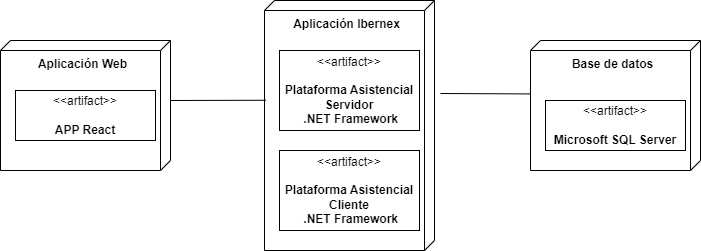
\includegraphics[width=0.8\textwidth,height=6cm]{Imagenes/Arquitectura_Sistema}
    \caption{Diagrama de despliegue}
    \label{fig:despliegue}
\end{figure}

La arquitectura completa respecto a lo que ha estado relacionado con el proyecto es la que se ve en la figura. No obstante lo que se ha implementado ha sido completamente la aplicación web y por otro lado se ha modificado y añadido funcionalidad a la Plataforma Asistencial Servidor de la aplicación de Ibernex. \newline

El ámbito del despliegue del sistema será en una red de área local (LAN) ya que serviría para una residencia u hospital en el que se instalaría el sistema configurando la base de datos correspondiente a la información de los pacientes del centro. \newline


TODO: Terminar de explicar la arquitectura final del sistema consultando con Carlos para hacerlo correctamente respecto a la parte de Ibernex\\

% Explicar que yo mayormente trabajo con PAServidor y qé es, que PACliente no lo toco para nada pero está dentro de la app y para qué lo utilizo.

% Añadir los terminales en el diagrama conectándolo con la aplicación de Ibernex.

% Hacer referencia al Anexo donde se expliquen las alternativas que se plantearon
La arquitectura aquí expuesta es la elegida entre las distintas opciones barajadas que se pueden ver con detalle en el \hyperref[anexo-a]{Anexo A}.


\section{Base de datos}

% Explicar qué partes de la base de datos utilizo de su sistema y con diagramas

TODO: explicar qué tablas de la base de datos utilizo de su sistema y adjuntaré  diagramas creados con la aplicación Microsoft SQL Server Management. \\

% INCLUIR EN EL ESQUEMA DEL LOGIN LA TABLA DE LOS RECURSOS DONDE ESTARÁN LOS PUESTOS

% REVISAR EL RESTO DE DIAGRAMAS PARA QUE REALMENTE ESTÉ TODO LO QUE SE HA UTILIZADO

\section{Interfaz de usuario}

% Poner la interfaz final del usuario cuando esté terminada

TODO: Poner la interfaz final del usuario cuando esté terminada

